% Seção 6: Conclusão

\section{Conclusão}
\begin{frame}
    \frametitle{Conclusão}
    \begin{itemize}
        \item A integração SDN/NVF/5G é a base da transformação digital
        \item Flexibilidade e agilidade
        \begin{itemize}
            \item SDN: Controle centralizado e programável da rede.
            \item NFV: Virtualização de funções de rede para rápida implantação e escalabilidade.
        \end{itemize}
        \item Redução de Custos Operacionais
        \begin{itemize}
            \item Menor dependência de hardware proprietário, redução de OPEX e CAPEX.
        \end{itemize}
        \item Automação e Controle em Tempo Real
        \begin{itemize}
            \item SDN: Automação e otimização do tráfego em tempo real.
            \item NFV: Implantação rápida e ajuste de serviços conforme as condições de rede.
        \end{itemize}
        \item Dicas valiosas a seguir...
    \end{itemize}
\end{frame}

\begin{frame}
    \frametitle{Dicas Valiosas}
    \begin{columns}
        \begin{column}{0.6\linewidth}
            \begin{itemize}
                \item Aprenda a desenvolver software \\
                \vspace{1cm}
                {\small
                ``We reject: kings, presidents, and voting. We believe in: rough consensus and running code.'' David Clark, 1992.
                }
                % \item Identificar tópicos quentes de pesquisa \\
                % {\small CFPs, acompanhar grupos de pesquisa, trabalhos futuros de teses e dissertações etc.}
                % \item Publicar é muito importante \\ 
                % {\small (\textit{Publish or perish}!!)}
                % \item Não brigue com seu orientador \\
                % {\small (Apesar de não ser um Jedi, respeite a opnião dele e dos mais experientes)}
                % \item A caminhada é muitas vezes mais rica do que o final da trilha
            \end{itemize}
        \end{column}
        \begin{column}{0.5\linewidth}
            \begin{figure}
                \centering
                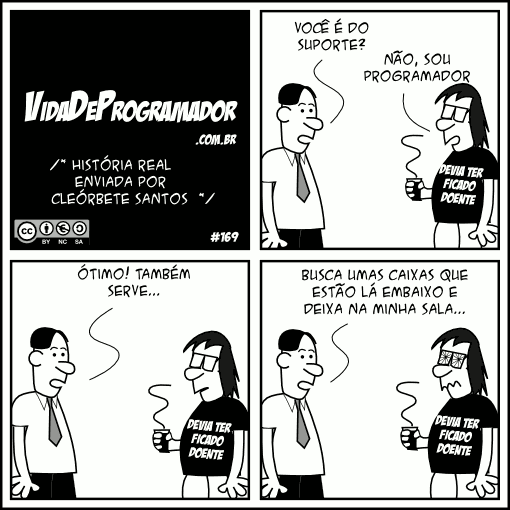
\includegraphics[width=\linewidth]{figs/vida_programador_tirinha169.png}
                \caption{\href{https://developerslife.tech/pt/2011/07/12/voce-e-do-suporte/}{Vida de programador \#169}}
            \end{figure}
        \end{column}
    \end{columns}    
\end{frame}

\begin{frame}
    \frametitle{Dicas Valiosas}
        \begin{itemize}
            \item Identificar tópicos quentes de pesquisa \\
            \vspace{0.5cm}
            {\small CFPs, acompanhar grupos de pesquisa, trabalhos futuros de teses e dissertações etc.}
            % \item Publicar é muito importante \\ 
            % {\small (\textit{Publish or perish}!!)}
            % \item Não brigue com seu orientador \\
            % {\small (Apesar de não ser um Jedi, respeite a opnião dele e dos mais experientes)}
            % \item A caminhada é muitas vezes mais rica do que o final da trilha
        \end{itemize}
        \begin{figure}
            \centering
            
\includegraphics[width=\linewidth]{figs/phdcomics.png}
            \caption{\href{https://phdcomics.com/comics/archive_print.php?comicid=1672}{PhD Comics: ``Professed?''}}
        \end{figure}
\end{frame}

\begin{frame}
    \frametitle{Dicas Valiosas}
        \begin{itemize}
            \item Publicar é muito importante (\textit{publish or perish}!!)
            % \item Não brigue com seu orientador \\
            % {\small (Apesar de não ser um Jedi, respeite a opnião dele e dos mais experientes)}
            % \item A caminhada é muitas vezes mais rica do que o final da trilha
        \end{itemize}
        \begin{figure}
            \centering
            
\includegraphics[width=0.8\linewidth]{figs/thesis_defense.png}
            \caption{\href{https://www.explainxkcd.com/wiki/index.php/1403:_Thesis_Defense}{Explain xkcd}}
        \end{figure}
\end{frame}

\begin{frame}
    \frametitle{Dicas Valiosas}
        \begin{itemize}
            \item Não brigue com seu orientador \\
            {\small (Apesar de não ser um Jedi, respeite a opnião dele e dos mais experientes)}
            % \item A caminhada é muitas vezes mais rica do que o final da trilha
        \end{itemize}
        \begin{figure}
            \centering
            
\includegraphics[width=0.8\linewidth]{figs/Obi-Wan-and-Anakin.png}
            \caption{\href{https://screenrant.com/star-wars-obi-wan-left-anakin-to-die-reason/}{Screen Rant}}
        \end{figure}
\end{frame}

\begin{frame}
    \frametitle{Dicas Valiosas}
        \begin{itemize}
            \item Registre tudo (escrita), não deixe pra depois \\
            (Principalmente os resultados e as revisões de trabalhos relacionados!!)
            \item Faça reuniões constantes
            % \item A caminhada é muitas vezes mais rica do que o final da trilha
        \end{itemize}
        \begin{figure}
            \centering
            
\includegraphics[width=0.3\linewidth]{figs/dory.jpg}
            \caption{\href{https://www.deviantart.com/the-avenged-evil/art/Finding-Nemo-Dory-325470391}{Deviant Art}}
        \end{figure}
\end{frame}

\begin{frame}
    \frametitle{Dicas Valiosas}
        \begin{itemize}
            \item A caminhada é muitas vezes mais rica do que o final da trilha
            \item O processo de formação do profissional é talvez mais importante do que o documento final
        \end{itemize}
        \begin{figure}
            \centering
            
\includegraphics[width=0.3\linewidth]{figs/magicodeoz.jpg}
            \caption{\href{https://www.thymindoman.com/the-mysticism-of-the-wizard-of-oz-our-journey-home/}{Thy Mind O Man}}
        \end{figure}
\end{frame}